\section[LVCS]{Letter based Visual Cryptographic Scheme}
Éste algoritmo es el que se propone en \textsl{Hsiao-Ching Lin et
al}\cite{articulo_base}. Es idéntico a los algoritmos DVCS y PVCS que hemos
visto, solo que cambian los píxeles por letras, de manera que dos letras
distintas superpuestas van a enegrecer el superpíxel, mientras que dos letras
superpuestas iguales se verán más blancuzcas.

\subsection{Transformación de matrices base}
Para sustituir los píxeles por letras hay que modificar las matrices base
cambiando los 0s y 1s por letras. Para ello vamos a seguir el algoritmo
\ref{alg:transf_matrices_base}.

\begin{algorithm}[H]
	\KwIn{\\Una matriz base binaria $B$ de $N\times m$}
	\KwResult{\\Una matriz de letras $L$ de $N\times m$ letras}

	1. Elegir un vector $R$ de $m$ letras, que representará los 0s de
	nuestra matriz

	\tcc{Recorremos los elementos de la matriz base. $(i,j)$ es la posición
		de $e_{i,j}$ en la matriz $B$}
	\For{all elements $e_{i,j}$ in $B$}{
		\eIf{$e_{i,j}$ == 0}{
			\tcc{Sustituimos por la misma letra que el representante
			de esa columna}
			$L[i][j] = R[j]$
		}{
			\tcc{Sustituimos por una letra aleatoria a todas las de
			la columna (incluido el representante)}
			$L[i][j] = L | L != L[k][j] \wedge L != R[j] con k \in
			[0,N-1]$
		}
	}
	\Return{$L$}
	\caption{Algoritmo de transformación de matrices base binarias a
	matrices base de letras}
	\label{alg:transf_matrices_base}
\end{algorithm}

A continuación mostramos un ejemplo de aplicación del algoritmo:
\begin{align}
	\nonumber
	\text{Vector representante = }
	&\begin{bmatrix}
		A & B & C\\
	\end{bmatrix}
	\\\nonumber
	&\begin{bmatrix}
		1 & 0 & 0\\
		0 & 1 & 0\\
		0 & 0 & 1
	\end{bmatrix}
	\rightarrow
	\begin{bmatrix}
		D & B & C\\
		A & F & C\\
		A & B & G
	\end{bmatrix}
\end{align}

\subsection{Mejoras}
El artículo de \textsl{Hsiao-Ching et al}\cite{articulo_base} propone cierta
mejora en la calidad del resultado del algoritmo, basada en la elección de
determinadas matrices base. Además, nosotros hemos introducido otra mejora en la
transformación de matrices base binarias a matrices de letras. Estas dos mejoras
las explicamos en las siguientes secciones.

\subsubsection{Condición de seguridad}
La condición de seguridad que explicábamos en \refcont{sec:matrices_base}
(equación \ref{eq:cond_seguridad}) tiene una excepción al pasar las matrices
binarias a matrices de letras. Esto es debido a que no es posible calcular la
distancia de hamming a una fila de letras, mientras que sí lo es en una de
píxeles. Un ``píxel'' negro con letras viene representado por una superposición
de letras distintas, y uno blanco por letras iguales, así que no tiene sentido
el concepto de ``píxel'' cuando no hay superposición. Por lo tanto podemos
admitir que la condición de seguridad siempre se cumple para $r=1$, ya que una
sola sombra de letras no puede revelar información sobre la imagen encriptada (a
excepción de lo que explicamos en la próxima sección).

La mejora que proponen se basa en esta propiedad para construir matrices base en
las que $B_0$ es una matriz de ``0s'', es decir, con letras iguales en todas sus
columnas. Aunque esto no cumpliría la restricción de seguridad para los
algoritmos DVCS y PVCS, si lo hace para LVCS, y además mejora notablemente la
calidad de las imágenes resultantes en esquemas $(2,N)$, ya que los blancos son
representados en su totalidad por letras superpuestas iguales. En las figuras
\ref{fig:LVCS_comparacion} se muestra la diferencia entre una imagen resultado
con la mejora y sin ella.

\begin{figure}[hp]
	\centering
	\begin{subfigure}[t]{0.9\textwidth}
		\centering
		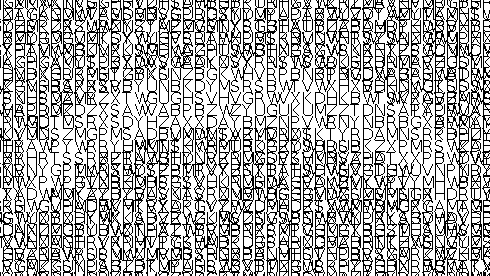
\includegraphics[width=\textwidth]{images/matriz_mejorada}
		\caption{Resultado con mejora}
	\end{subfigure}
	\\[0.5cm]
	\begin{subfigure}[t]{0.9\textwidth}
		\centering
		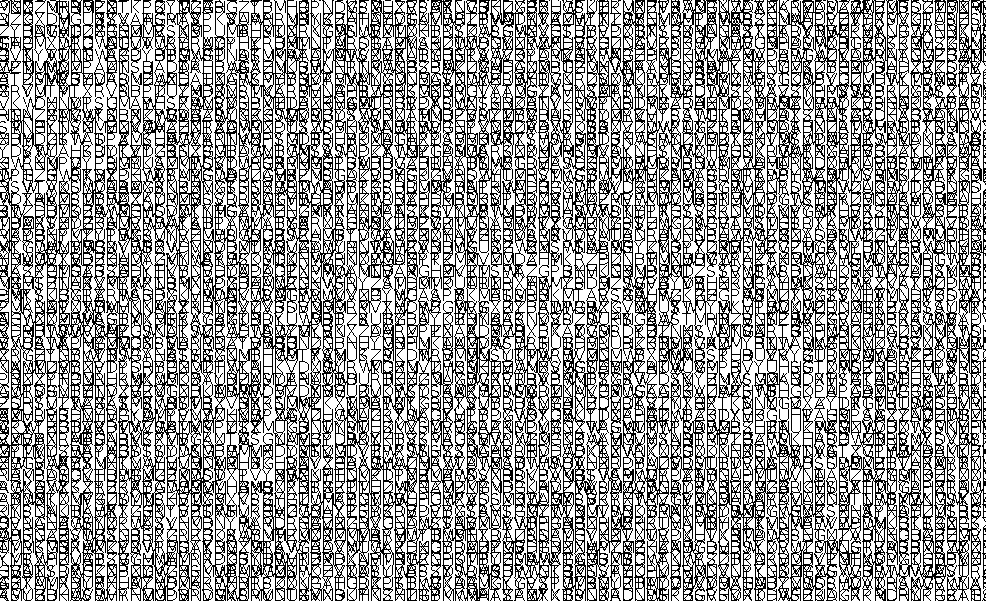
\includegraphics[width=\textwidth]{images/matriz_sin_mejora}
		\caption{Resultado sin mejora}
	\end{subfigure}
	\caption{Comparación de un cifrado con matrices base mejoradas y sin
	mejorar.}
	\label{fig:LVCS_comparacion}
\end{figure}

\subsubsection{Reelección de representantes}
Al transformar una matriz base binaria a una de letras, si para todos los
superpíxeles que generamos elegimos el mismo representante para $B_0$ y otro
distinto para $B_1$, el usar letras diferentes para representar el negro y el
blanco, hace que podamos apreciar la imagen encriptada con una sola sombra. Esto
se soluciona eligiendo un representante aleatorio distinto cada vez que tenemos
que generar un nuevo superpíxel, siempre y cuando usemos el mismo para todas las
sombras. En las figuras \ref{fig:LVCS_representantes} se muestra el problema.

Aunque las imágenes que se muestran en el artículo \cite{articulo_base} parecen
tener en cuenta este hecho, el algoritmo que se propone no lo describe.

\begin{figure}[hp]
	\centering
	\begin{subfigure}[t]{0.8\textwidth}
		\centering
		
\includegraphics[width=\textwidth]{images/rep_mejorado}
		\caption{Resultado con mejora}
	\end{subfigure}
	\\[0.5cm]
	\begin{subfigure}[t]{0.8\textwidth}
		\centering
		
\includegraphics[width=\textwidth]{images/rep_sin_mejora}
		\caption{Resultado sin mejora}
	\end{subfigure}
	\\[0.5cm]
	\begin{subfigure}[t]{0.2\textwidth}
		\centering
		
\includegraphics[width=\textwidth]{images/rep_original}
		\caption{Imagen original}
	\end{subfigure}
	\caption{Comparación de dos sombras, una con reelección de
	representantes y otra sin reelección}
	\label{fig:LVCS_representantes}
\end{figure}
